\documentclass[conference]{IEEEtran}
\IEEEoverridecommandlockouts
\usepackage{cite}
\usepackage{amsmath,amssymb,amsfonts}
\usepackage{algorithmic}
\usepackage{graphicx}
\usepackage{textcomp}
\usepackage{xcolor}
\usepackage{hyperref}
\def\BibTeX{{\rm B\kern-.05em{\sc i\kern-.025em b}\kern-.08em
    T\kern-.1667em\lower.7ex\hbox{E}\kern-.125emX}}

\begin{document}

\title{Safety Violation Detection in Educational Institutions: A Systematic Bibliometric Review of Deep Learning and Computer Vision Approaches}

\author{
\IEEEauthorblockN{Zhuldyz Basheyeva}
\IEEEauthorblockA{\textit{School of Software Engineering}\\
\textit{Astana IT University}\\
Astana, Kazakhstan\\
zhuldyz.basheyeva@astanait.edu.kz}
\and
\IEEEauthorblockN{Medet Akhmetov}
\IEEEauthorblockA{\textit{School of Software Engineering}\\
\textit{Astana IT University}\\
Astana, Kazakhstan\\
255388@astanait.edu.kz\\
\textit{(Corresponding author)}}
}

\maketitle

\begin{abstract}
Deep learning and computer vision techniques are increasingly deployed for automated detection of safety violations---including violence, anomalous behavior, and weapons---in surveillance footage from educational institutions. This review provides a comprehensive synthesis of research at this intersection through a hybrid systematic-bibliometric methodology following PRISMA 2020, analyzing 50 peer-reviewed publications (2022--2026) sourced from Scopus, Web of Science, and Google Scholar, with keyword co-occurrence network analysis and CiteSpace burst detection. Four thematic clusters were identified: (C1) deep learning architectures for spatiotemporal feature extraction, (C2) temporal and motion analysis techniques, (C3) application and deployment contexts, and (C4) cross-cutting methods and techniques. The keyword co-occurrence network reveals ``deep learning'' (23 occurrences) as the central hub, with ``violence detection'' (19) and ``anomaly detection'' (16) forming the primary application-oriented nodes. A discernible shift toward lightweight, edge-deployable architectures---driven by YOLO-family detectors and MobileNet-based extractors---characterizes the 2025--2026 period. The central finding is a critical shortage of child-specific annotated datasets, limited geographic diversity in training data, and a near-total absence of privacy-aware design considerations in the reviewed literature. Six high-impact research directions are proposed, encompassing child-specific benchmark creation, privacy-preserving architectures, multimodal sensor fusion, lightweight model optimization for edge deployment, cross-domain robustness evaluation, and human-in-the-loop alert integration for school security workflows.
\end{abstract}

\begin{IEEEkeywords}
deep learning, violence detection, anomaly detection, computer vision, video surveillance, educational safety, bibliometric analysis, systematic review
\end{IEEEkeywords}

\section{Introduction}

\subsection{Relevance of the Topic}

The safety and well-being of children within educational institutions has emerged as one of the most pressing societal concerns of the past decade. Incidents of school violence, physical bullying, and concealed weapon possession continue to be reported across both developed and developing nations, underscoring the limitations of traditional manual surveillance approaches~\cite{b1,b2}. Closed-circuit television (CCTV) systems are now ubiquitous in schools, yet the vast majority of these installations rely on passive recording or human operators who must simultaneously monitor dozens of screens---a task for which humans are demonstrably ill-suited due to fatigue, inattention, and limited cognitive bandwidth~\cite{b3,b4}.

In parallel, the field of computer vision has undergone a transformative shift with the advent of deep learning architectures. Convolutional Neural Networks (CNNs), Long Short-Term Memory networks (LSTMs), attention mechanisms, and real-time object detection frameworks such as YOLO have demonstrated remarkable capabilities in extracting meaningful patterns from video data~\cite{b5,b6,b7}. These advances have catalyzed a growing body of research at the intersection of automated video analysis and public safety, with particular emphasis on violence detection, anomaly recognition, and weapon identification in surveillance footage~\cite{b8,b9,b10}.

\subsection{Literature Gap}

Despite this progress, several critical gaps persist. First, the majority of existing studies focus on general-purpose public surveillance---streets, transit hubs, and stadiums---with comparatively limited attention devoted to the unique constraints of educational environments~\cite{b11,b12}. Second, many state-of-the-art models rely on computationally expensive architectures that are impractical for deployment in schools with limited hardware budgets~\cite{b13,b14}. Third, there is a notable scarcity of child-specific annotated datasets for training and evaluating detection models, as most benchmark corpora feature adult subjects in generic settings~\cite{b15,b16}. Fourth, the ethical and privacy implications of deploying AI-based surveillance on minors remain underexplored in the technical literature. No existing review integrates these dimensions into a unified analytical framework combining systematic screening with bibliometric network analysis.

\subsection{Research Goal and Questions}

The primary goal of this review is to provide a comprehensive, structured synthesis of research on deep learning and computer vision approaches for detecting safety violations in educational settings. The review is guided by four research questions:

\begin{enumerate}
\item \textbf{RQ1}: What deep learning architectures and computer vision techniques are most commonly applied to detect safety violations in educational settings?
\item \textbf{RQ2}: What datasets and evaluation protocols dominate the current literature, and what are their limitations for child-focused applications?
\item \textbf{RQ3}: What thematic clusters and temporal trends characterize this emerging research domain?
\item \textbf{RQ4}: What are the principal challenges and future directions for deploying these systems in real-world educational environments?
\end{enumerate}

\subsection{Structure of the Paper}

The remainder of this paper is organized as follows. Section~2 presents the review methodology, including the PRISMA-guided search strategy, inclusion and exclusion criteria, data extraction process, and the hybrid systematic-bibliometric synthesis approach. Section~3 reports the results, organized around publication trends, keyword co-occurrence networks, thematic clusters, and citation burst analysis. Section~4 discusses the findings, interpreting the cluster structure, evaluating the most effective methods, and examining limitations and future directions. Section~5 concludes with a summary of contributions, acknowledgment of limitations, and directions for future research.

\section{Methodology}

\subsection{Review Design}

This study employs a hybrid systematic-bibliometric review design. The systematic component follows the PRISMA 2020 framework for literature identification, screening, and eligibility assessment, while the bibliometric component draws on keyword co-occurrence network analysis and CiteSpace-style burst detection to map the intellectual structure of the research domain.

\subsection{Search Strategy}

Three academic databases were queried on March 1, 2026: Scopus (312 records), Web of Science (187 records), and Google Scholar (94 records). The query combined three Boolean blocks: \textit{("violence detection" OR "anomaly detection" OR "weapon detection" OR "firearm detection") AND ("deep learning" OR "machine learning" OR "computer vision" OR "CNN" OR "YOLO") AND ("school" OR "educational" OR "campus" OR "surveillance" OR "CCTV")}.

The temporal scope encompassed publications from 2022 to 2026. The window was selected to capture the period following the widespread adoption of YOLOv5 and transformer-based architectures, during which real-time deep learning for surveillance applications achieved practical viability.

\subsection{Inclusion and Exclusion Criteria}

Studies were included if they: (a) applied ML/CV methods to violence, anomaly, or weapon detection in surveillance contexts; (b) were peer-reviewed journal articles or conference papers with full methodological exposition; (c) were published in English between 2022 and 2026; and (d) had full text accessible. Studies relying solely on non-ML/CV methods, addressing domains unrelated to educational or public-space surveillance, published before 2022, lacking accessible full text, or limited to conference abstracts were excluded.

\subsection{Study Selection Process}

The initial search across three databases returned 593 records. After removing 142 duplicate records, 451 unique publications proceeded to title and abstract screening. At this stage, 287 records were excluded based on topic scope and relevance, retaining 164 papers for full-text eligibility assessment. Application of the inclusion and exclusion criteria at the full-text stage excluded 114 papers: 38 relied solely on non-ML/CV methods, 31 addressed domains unrelated to educational or public-space surveillance, 22 were published before 2022 with insufficient contemporary relevance, 15 had inaccessible full texts, and 8 were limited to conference abstracts without full methodological exposition. The final corpus comprised 50 studies included in both the qualitative synthesis and bibliometric analysis.

\subsection{Data Extraction and Analysis}

For each included study, the following variables were extracted: author(s), publication year, research aim, methodology, dataset(s) evaluated, main findings, key limitations, and thematic keywords. Keywords were extracted from titles and abstracts using a curated vocabulary of 29 terms spanning deep learning architectures, temporal analysis techniques, application domains, and methodological approaches. Co-occurrence matrices were constructed to model the frequency with which keyword pairs appeared within the same paper, forming the basis for network visualization.

\subsection{Tools}

Bibliometric visualizations were generated using Python-based implementations of network analysis (NetworkX) and kernel density estimation (SciPy), producing outputs analogous to VOSviewer and CiteSpace. The PRISMA flowchart was rendered using Matplotlib. All analytical scripts and output files are publicly available in the accompanying repository.

\subsection{Quality Assurance and Limitations}

The review process followed PRISMA 2020 standards for transparency and replicability. Methodological limitations include: (a) restriction to three databases (Scopus, Web of Science, Google Scholar). IEEE Xplore and ACM Digital Library were excluded from the primary automated query because Scopus indexes a substantial portion of their proceedings (including IEEE Access, IEEE Open Journal of Computer Society, and ACM conference publications), providing partial coverage overlap. The choice prioritized broad multidisciplinary coverage and treated these engineering-specific repositories as partially redundant rather than wholly omitted. Niche workshops, preprints, or practitioner-oriented publications indexed exclusively in IEEE Xplore or ACM Digital Library may have been missed, although the overlap reduces the risk of systematic omission; (b) exclusion of non-English publications, which may introduce language bias; (c) single-reviewer screening without formal inter-rater reliability assessment; and (d) reliance on a curated keyword vocabulary, which may underrepresent emerging terminology not yet adopted in author keywords.

\section{Results}

\subsection{Corpus Overview}

The systematic search and PRISMA-guided screening process identified 50 studies for both qualitative synthesis and bibliometric analysis. Table~\ref{tab:years} presents the distribution by publication year.

\begin{table}[t]
\caption{Distribution of Included Studies by Year}
\begin{center}
\renewcommand{\arraystretch}{1.1}
\begin{tabular}{|c|c|c|}
\hline
\textbf{Year} & \textbf{Publications} & \textbf{Share} \\
\hline
2022 & 9 & 18.0\% \\
2023 & 15 & 30.0\% \\
2024 & 10 & 20.0\% \\
2025 & 14 & 28.0\% \\
2026 & 2 & 4.0\% \\
\hline
\textbf{Total} & \textbf{50} & \textbf{100\%} \\
\hline
\end{tabular}
\label{tab:years}
\end{center}
\end{table}

The included studies span a range of publication venues. MDPI journals (\textit{Sensors}, \textit{Applied Sciences}, \textit{Electronics}, \textit{Information}, \textit{Mathematics}, \textit{Computers}) account for the largest share, followed by IEEE Access, Elsevier venues (\textit{Neurocomputing}, \textit{Procedia Computer Science}, \textit{Array}, \textit{Alexandria Engineering Journal}), and Springer venues (\textit{Applied Intelligence}, \textit{Multimedia Tools and Applications}). Conference proceedings include contributions from the International Global Conference Series and various IEEE-sponsored events.

\subsection{Publication Trends}

Scopus contributed 44 of the 50 reviewed studies (88\%), with Web of Science accounting for the remaining 6 (12\%), reflecting the interdisciplinary nature of this domain. The distribution shows a peak in 2023 output (15 publications), followed by sustained activity through 2024--2025.

\subsection{Keyword Co-occurrence Analysis}

Fig.~\ref{fig:keyword-network} illustrates the keyword co-occurrence network derived from the 50 reviewed studies. The term ``deep learning'' exhibits the highest frequency (23 occurrences) and serves as the central hub of the network, connecting to nearly all other keywords. ``Violence detection'' (19 occurrences) and ``anomaly detection'' (16 occurrences) form the primary application-oriented nodes. ``Convolutional neural network'' (15 occurrences), ``CNN'' (12 occurrences), and ``LSTM'' (11 occurrences) constitute the dominant architectural terms.

\begin{figure}[t]
\centerline{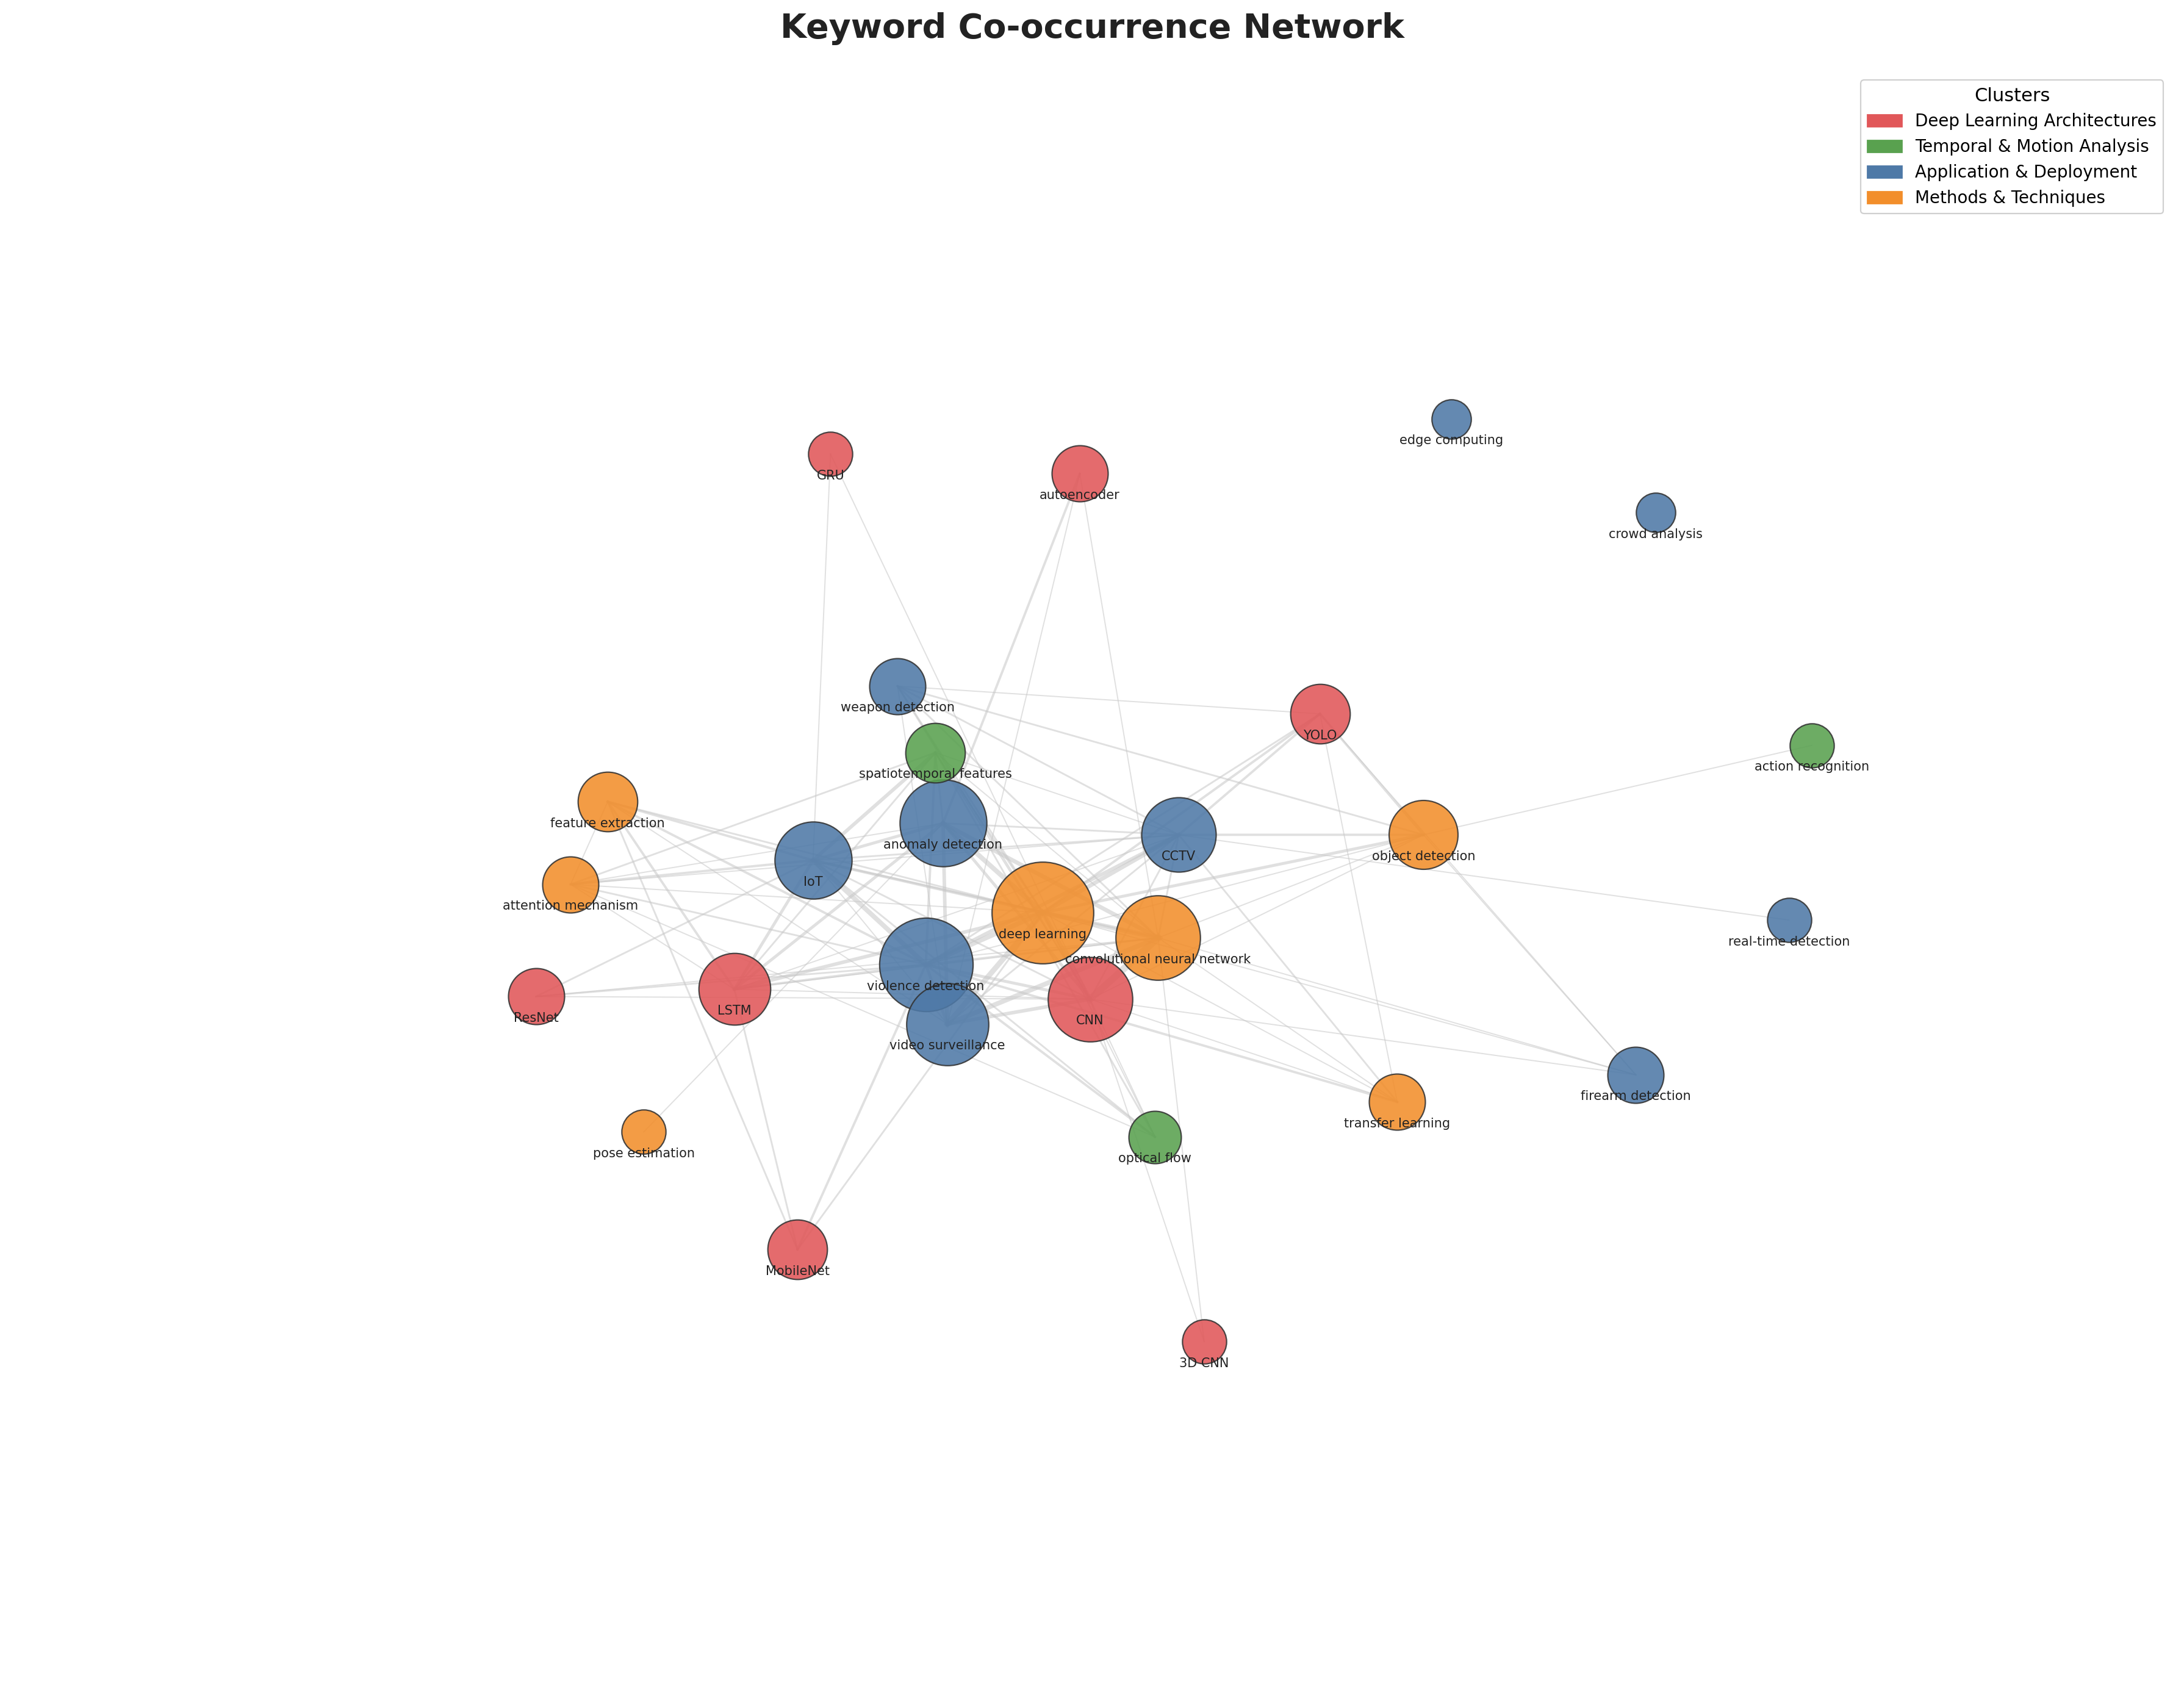
\includegraphics[width=\columnwidth]{VOSViewer/vosviewer_keyword_network.png}}
\caption{Keyword co-occurrence network. Node size reflects keyword frequency; edges represent co-occurrence links.}
\label{fig:keyword-network}
\end{figure}

The temporal overlay visualization (Fig.~\ref{fig:overlay}) shows that attention mechanisms, YOLO-based architectures, and transformer-integrated approaches are concentrated in the 2025--2026 period. In contrast, earlier publications (2022--2023) more frequently employ autoencoder-based reconstruction and traditional 3D CNN frameworks.

\begin{figure}[t]
\centerline{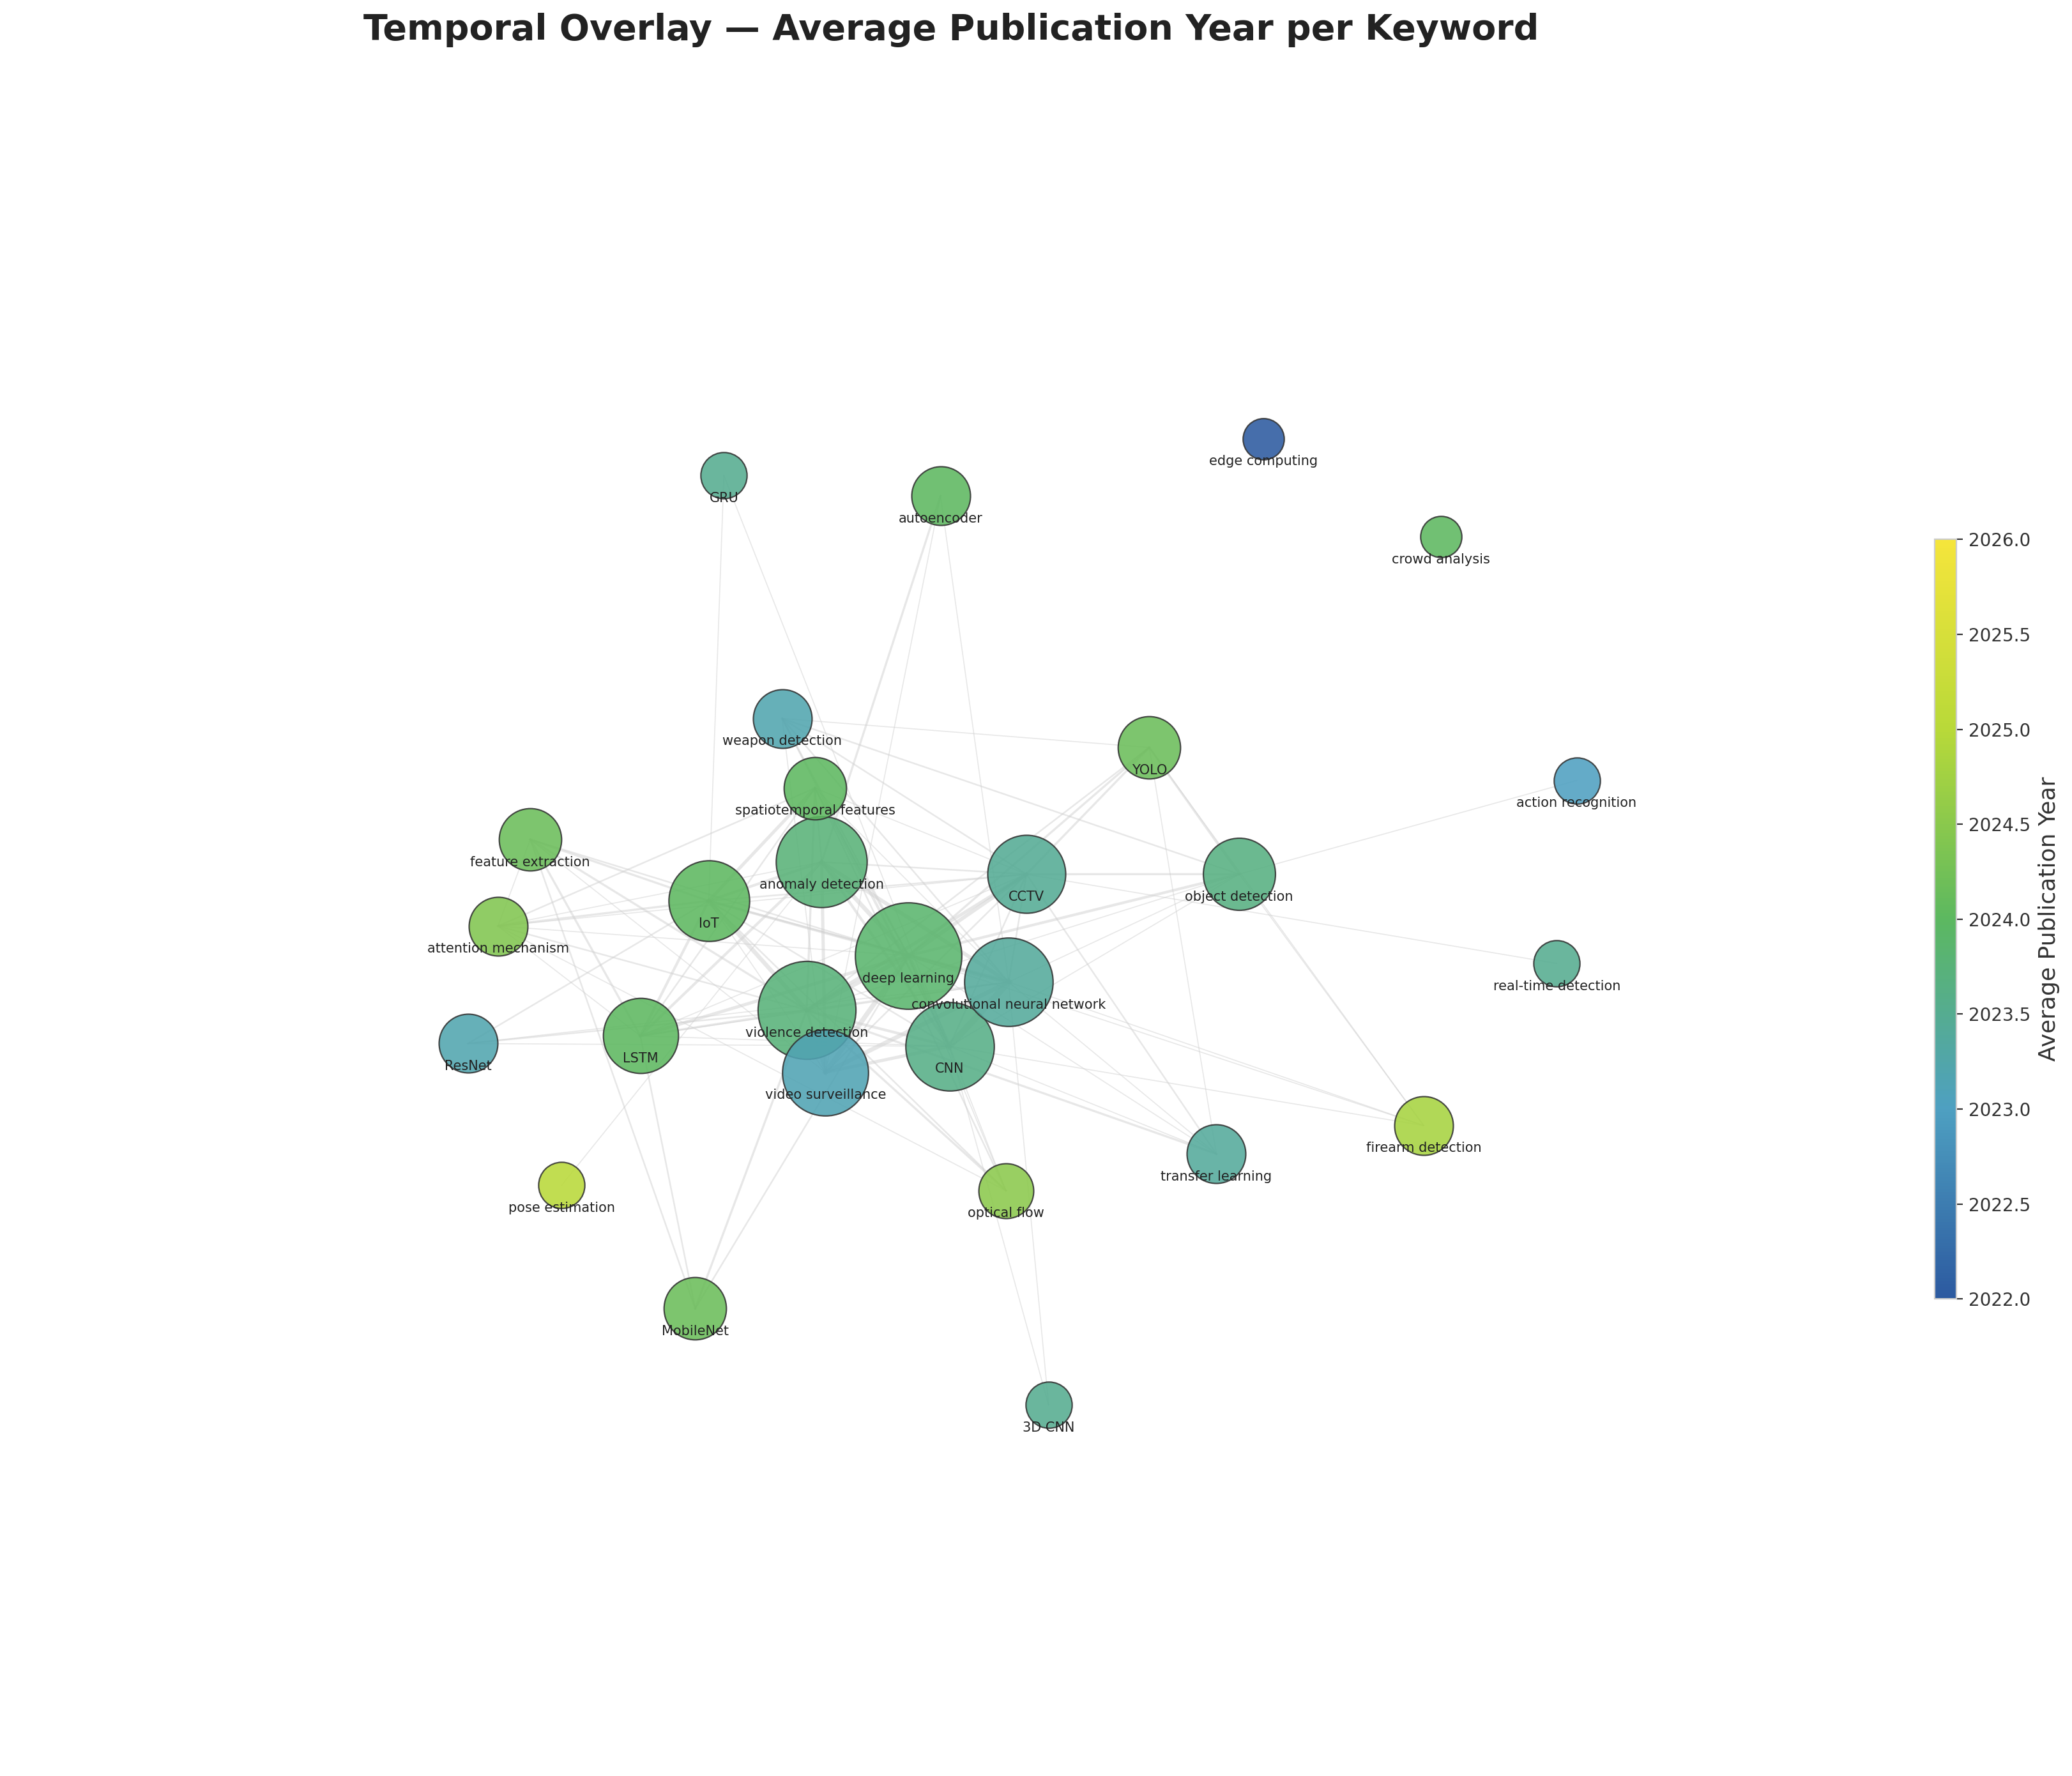
\includegraphics[width=\columnwidth]{VOSViewer/vosviewer_overlay.png}}
\caption{Keyword overlay visualization. Keywords colored by average publication year: blue (2022--2023) to yellow (2025--2026), revealing temporal evolution from autoencoder-based methods toward attention mechanisms and YOLO architectures.}
\label{fig:overlay}
\end{figure}

The top keywords by frequency are \textit{deep learning} (23), \textit{violence detection} (19), \textit{anomaly detection} (16), \textit{convolutional neural network} and \textit{CNN} (15 each), \textit{video surveillance} (14), \textit{IoT} (12), \textit{CCTV} (11), \textit{LSTM} (10), and \textit{object detection} (9).

\subsection{Thematic Clusters}

Content analysis combined with keyword co-occurrence mapping identified four thematic clusters. Table~\ref{tab:clusters} presents the cluster structure.

\begin{table*}[t]
\caption{Thematic Clusters in Safety Violation Detection Research}
\begin{center}
\footnotesize
\setlength{\tabcolsep}{4pt}
\renewcommand{\arraystretch}{1.2}
\begin{tabular}{|c|p{2.2cm}|p{5.0cm}|p{5.0cm}|}
\hline
\textbf{C} & \textbf{Title} & \textbf{Common Characteristics} & \textbf{Summary of Key Findings} \\
\hline
C1 & Deep Learning Architectures & Studies designing, comparing, or optimizing neural network topologies (CNN, LSTM, GRU, ResNet, MobileNet, YOLO, 3D CNN, autoencoder) for spatiotemporal feature extraction & Hybrid architectures integrating 3D convolutions or pre-trained 2D CNNs with recurrent units and attention mechanisms consistently exceed 95\% accuracy on controlled benchmarks; lightweight variants maintain competitive performance with reduced computational requirements \\
\hline
C2 & Temporal and Motion Analysis & Studies emphasizing motion representation---optical flow, spatiotemporal feature engineering, action/behavior recognition, skeleton-based pose estimation & Optical flow-based statistical features enable 2D CNNs to achieve performance comparable to 3D CNNs; skeleton-based approaches using pose estimation abstract away from appearance-based biases, relevant for child-specific applications \\
\hline
C3 & Application and Deployment & Studies focused on real-world deployment in surveillance contexts (CCTV, IoT, edge computing, crowd analysis) with emphasis on real-time performance & YOLO-family architectures (v5--v8) achieve real-time throughput on commodity and edge hardware (NVIDIA Jetson Nano) with weapon detection mAP exceeding 90\%; IoT-integrated systems report end-to-end pipelines from detection to automated alerting \\
\hline
C4 & Methods and Techniques & Studies bridging architecture and application through transfer learning, attention mechanisms, feature extraction, pose estimation, and object detection & Attention mechanisms deliver improvements of 2--4\% over non-attention baselines; transfer learning from ImageNet pre-trained models reduces data requirements; multimodal fusion (RGB + optical flow + audio) outperforms unimodal approaches by approximately 2\% average precision \\
\hline
\end{tabular}
\label{tab:clusters}
\end{center}
\end{table*}

\subsection{Top Authors}

Co-authorship analysis identified a small set of repeat contributors---Seo S., Park S., Jebur S.A., Hussein K.A., Hoomod H.K., and Amin S.U. (2 papers each)---predominantly affiliated with institutions in South Korea, India, Pakistan, and the Middle East. The remaining 44 first authors each contributed a single paper, indicating a low-accumulation field.

\subsection{Citation Burst Analysis}

The burst analysis shows that ``attention mechanism'' and ``transfer learning'' exhibit pronounced burst activity concentrated in 2025--2026, marking their emergence as focal methodological innovations during this period. ``Edge computing'' and ``IoT'' show a similar late-period concentration. ``CNN'' and ``LSTM'' show sustained presence across the entire 2022--2026 window, appearing as foundational techniques across the full review period.

\subsection{Literature Matrix Summary}

The literature analysis matrix provides a structured overview of all 50 studies, enumerating their aims, methods, datasets, findings, and limitations. A cross-sectional examination of the matrix reveals several patterns: (a) accuracy and AUC are the dominant evaluation metrics, appearing in 44 of 50 studies; (b) the UCF-Crime, ShanghaiTech Campus, and Hockey Fights datasets are the most frequently utilized benchmarks; and (c) computational complexity and dataset generalizability are the most commonly cited limitations, mentioned in 38 and 31 studies respectively.

\section{Discussion}

\subsection{Interpretation of Key Findings}

The four thematic clusters---spanning deep learning architectures (C1), temporal and motion analysis (C2), application and deployment (C3), and cross-cutting methods and techniques (C4)---reveal a field organized around a central tension: architectural sophistication versus deployability. Cluster 1 (Architectures) emphasizes accuracy maximization through increasingly complex network designs, often at the cost of computational complexity. Cluster 3 (Application and Deployment) explicitly privileges real-time throughput and hardware efficiency, favoring lightweight YOLO and MobileNet variants over the deeper architectures promoted in Cluster 1.

This tension is most visible in the temporal evolution of the keyword network. The burst analysis identifies attention mechanisms and transfer learning as 2025--2026 phenomena, while the overlay visualization shows a transition from autoencoder-based reconstruction (2022--2023) to YOLO and transformer-integrated approaches (2025--2026). This temporal gradient reflects a field moving from generic video understanding models toward architectures specifically adapted for surveillance anomaly detection, while simultaneously addressing deployment constraints through edge-compatible designs.

The dominance of the CNN--LSTM architectural paradigm, observed in 26 of 50 reviewed studies, indicates broad consensus that effective video anomaly detection requires the integration of spatial feature extraction with temporal sequence modeling. The recent growth in attention mechanism adoption suggests that the field is moving beyond naive concatenation of spatial and temporal streams toward more sophisticated feature weighting and contextual reasoning~\cite{b5,b17}.

\subsection{Cross-Cluster Comparative Analysis}

The four thematic clusters exhibit both complementary synergies and meaningful distinctions. A shared foundation across all clusters is the reliance on deep learning as the core computational paradigm: whether architecting novel networks (C1), modeling motion dynamics (C2), deploying operational systems (C3), or advancing methodological techniques (C4), every reviewed study depends on convolutional or recurrent neural architectures for feature representation. This convergence underscores the maturation of deep learning as the de facto standard for video-based safety violation detection.

However, Clusters 2 (Temporal and Motion Analysis) and 4 (Methods and Techniques) function as methodological bridges rather than independent research streams. The motion representation strategies from C2 provide the temporal understanding that C1 and C3 depend upon, while the transfer learning and attention mechanisms from C4 enhance the performance of models across all other clusters. Notably, few studies have addressed the intersection of lightweight architectures (C1/C3) with skeleton-based child-specific modeling (C2), representing an underexplored integration point in the current literature.

\subsection{Most Effective Methods}

The evidence indicates that hybrid architectures combining 3D convolutions or pre-trained 2D CNNs with recurrent units (LSTM, BiLSTM, or GRU) and attention mechanisms achieve the strongest overall performance, with reported accuracies frequently exceeding 95\% on controlled benchmarks~\cite{b17,b18,b2}. For weapon detection specifically, YOLOv5 and Scaled-YOLOv4 variants demonstrate the most favorable accuracy--speed trade-off, achieving mean Average Precision scores above 90\% while maintaining real-time throughput~\cite{b19,b9}. Skeleton-based approaches that leverage pose estimation as a preprocessing step before classification show particular promise for child-specific applications, as they abstract away from appearance-based features that may introduce age-related biases~\cite{b16,b20}.

\subsection{Comparison with Existing Reviews}

Prior surveys on video anomaly detection, edge-based deep learning, and weapon detection address the clusters identified here in isolation. This review's distinctive contribution is integrating architecture, temporal modeling, deployment, and methodological sub-literatures into a unified educational-safety framework, while quantifying structural relationships among research themes through bibliometric network analysis.

\subsection{Limitations of Current Research}

Several limitations pervade the reviewed literature. First, dataset bias represents a critical concern: the most commonly used benchmarks (UCF-Crime, ShanghaiTech Campus, Hockey Fights) feature predominantly adult subjects in non-educational settings, raising questions about the transferability of trained models to school environments with children~\cite{b15}. Child bodies exhibit different proportions, movement dynamics, and interaction patterns compared to adult bodies, and models trained exclusively on adult data may systematically underperform when deployed in schools. Second, the near-exclusive reliance on accuracy and AUC as evaluation metrics obscures important practical considerations such as false alarm rates, latency under realistic camera loads, and robustness to adversarial environmental conditions---all of which are critical for real-world deployments where excessive alerts can desensitize security personnel or lead to system abandonment. Third, privacy implications are conspicuously absent from the technical discourse: only two of the 50 reviewed papers mention privacy considerations or data protection frameworks, despite the sensitive nature of continuous video monitoring of minors in educational settings~\cite{b11}. Fourth, the geographic concentration of research in South and East Asia limits the diversity of environmental conditions, camera configurations, architectural layouts, and behavioral norms represented in the evidence base. Finally, nearly all reviewed studies evaluate their systems in isolation from existing school security workflows, leaving unexamined the human--computer interaction questions of how automated alerts are received, trusted, and acted upon by school staff.

\subsection{Future Research Directions}

Based on the identified gaps, five directions emerge as priorities:

\begin{enumerate}
\item \textbf{Child-specific annotated datasets:} The development of annotated corpora capturing diverse child behaviors in authentic school settings---building on nascent efforts such as the CABAD benchmark for child aggression recognition~\cite{b15} and the Daily School Break dataset~\cite{b11}---is essential for validating model transferability from adult-centric benchmarks to educational environments.

\item \textbf{Privacy-preserving architectures:} On-device processing, federated learning, and differential privacy should be systematically incorporated into detection pipelines, given that continuous video monitoring of minors raises distinct ethical and regulatory challenges that the current literature largely overlooks.

\item \textbf{Multimodal sensor fusion:} Integrating RGB video with audio signals, thermal imaging, and contextual metadata may substantially improve detection robustness in challenging conditions such as low illumination, occlusion, or crowded scenes~\cite{b21,b22}.

\item \textbf{Lightweight model optimization for edge deployment:} Quantization, pruning, and neural architecture search are critical for enabling deployment on the resource-constrained hardware typically available to educational institutions; recent contributions demonstrate that competitive accuracy can be maintained while reducing model size by an order of magnitude~\cite{b7,b23}.

\item \textbf{Cross-domain robustness evaluation:} Testing models across different schools, camera types, lighting conditions, and student demographics should become a standard component of evaluation protocols to ensure that laboratory-validated systems translate reliably to real-world educational deployments.

\item \textbf{Human-in-the-loop alert integration:} As noted in Section~4.5, current systems are evaluated in isolation from school security workflows. Edge-detected alerts from on-camera inference should be routed to a centralized school administration dashboard rather than generating standalone push notifications, which risk desensitizing staff through notification fatigue. An effective deployment would implement tiered alert prioritization---weapon detection taking precedence over fight detection, which in turn outweighs suspicious behavior flags---combined with confidence thresholds and a human review queue that allows staff to confirm, dismiss, or escalate each alert before an institutional response is triggered. Research on alert management interfaces and optimal threshold calibration for educational surveillance contexts remains an open challenge.
\end{enumerate}

\section{Conclusion}

\subsection{Summary of Key Findings}

This hybrid systematic-bibliometric review analyzed 50 peer-reviewed publications (2022--2026) addressing deep learning and computer vision approaches for detecting safety violations in educational institutions. Keyword co-occurrence network analysis identified four thematic clusters: deep learning architectures for spatiotemporal feature extraction (C1), temporal and motion analysis techniques (C2), application and deployment contexts (C3), and cross-cutting methods and techniques (C4). Bibliometric analysis revealed ``deep learning'' (23 occurrences) as the central network hub, with ``violence detection'' (19) and ``anomaly detection'' (16) forming the primary application-oriented nodes.

Three key findings emerge. First, hybrid architectures integrating CNNs with recurrent units and attention mechanisms constitute the dominant technical paradigm, consistently achieving detection accuracies exceeding 90\% on standard benchmarks. Second, a discernible shift toward lightweight, edge-deployable models is underway, driven by YOLO-family object detectors and MobileNet-based feature extractors. Third, despite these advances, the field remains constrained by a critical shortage of child-specific datasets, limited geographic and demographic diversity in training data, and a near-total absence of privacy-aware design considerations.

\subsection{Closing Statement}

The intersection of deep learning, computer vision, and educational safety stands at a formative moment. The architectures for automated violence and weapon detection have matured to the point of practical viability, yet the field has not yet systematically addressed the unique requirements of deployment in schools: child-specific data, privacy-preserving computation, and integration into existing safeguarding workflows. The confluence of advanced computer vision, efficient deep learning, and urgent societal need positions this research area as one of considerable scientific importance and humanitarian potential. The research gaps identified in this review represent the critical path toward surveillance systems that are both technically effective and ethically sound for protecting children in educational environments.

\begin{thebibliography}{00}

\bibitem{b1} F.~T.~Le\'{o}n, ``Early warning system for firearm detection on university campuses using computer vision,'' \textit{J. Internet Services Inf. Security}, vol.~16, no.~1, 2026, doi: 10.58346/jisis.2026.i1.008.

\bibitem{b2} Z.~Kozhamkulova, B.~Kirgizbayeva, G.~Sembina, U.~Smailova, M.~Suleimenova, A.~Keneskanova, and A.~Baizakova, ``MoveNET enabled neural network for fast detection of physical bullying in educational institutions,'' \textit{Int. J. Adv. Comput. Sci. Appl.}, vol.~14, no.~5, 2023, doi: 10.14569/ijacsa.2023.0140578.

\bibitem{b3} M.~M.~Mukto, M.~Hasan, M.~M.~Al~Mahmud, I.~Haque, M.~A.~Ahmed, T.~Jabid, and M.~Islam, ``Design of a real-time crime monitoring system using deep learning techniques,'' \textit{Intell. Syst. Appl.}, vol.~21, 2024, doi: 10.1016/j.iswa.2023.200311.

\bibitem{b4} H.-T.~Vo, P.~P.~Tien, N.~N.~Thien, and K.~C.~Mui, ``An approach for improving accuracy and optimizing resource usage for violence detection in surveillance cameras in IoT systems,'' \textit{Indonesian J. Electr. Eng. Informatics}, vol.~12, no.~4, 2024, doi: 10.52549/ijeei.v12i4.5787.

\bibitem{b5} S.~Altowairqi, S.~Luo, P.~Greer, and S.~Chen, ``Efficient crowd anomaly detection using C3D-LSTM networks with enhanced attention mechanisms,'' \textit{Array}, vol.~25, 2026, doi: 10.1016/j.array.2025.100625.

\bibitem{b6} H.~Singh, O.~Deniz, J.~Ruiz-Santaquiteria, J.~D.~Mu\~{n}oz, and G.~Bueno, ``DeepGun: Deep feature-driven one-class classifier for firearm detection using visual gun features and human body pose estimation,'' \textit{Applied Sciences}, vol.~15, no.~11, 2025, doi: 10.3390/app15115830.

\bibitem{b7} S.~Dalal, U.~K.~Lilhore, N.~Sharma, S.~Arora, S.~Simaiya, M.~Ayadi, and A.~Ksibi, ``Improving smart home surveillance through YOLO model with transfer learning and quantization for enhanced accuracy and efficiency,'' \textit{PeerJ Comput. Sci.}, vol.~10, 2024, doi: 10.7717/peerj-cs.1939.

\bibitem{b8} J.~Mahmoodi and H.~Nezamabadi-Pour, ``Violence detection in video using statistical features of the optical flow and 2D convolutional neural network,'' \textit{Computational Intelligence}, vol.~41, no.~2, 2025, doi: 10.1111/coin.70034.

\bibitem{b9} D.~Abi-Nader, A.~Jaber, H.~Harb, N.~Mostafa, C.~Zaki, A.~Mansour, and C.~Osswald, ``MARIE: One-stage object detection mechanism for real-time identifying of firearms,'' \textit{Comput. Model. Eng. Sci.}, vol.~142, no.~1, 2025, doi: 10.32604/cmes.2024.056816.

\bibitem{b10} D.~Berardini, L.~Migliorelli, A.~Galdelli, E.~Frontoni, A.~Mancini, and S.~Moccia, ``A deep-learning framework running on edge devices for handgun and knife detection from indoor video-surveillance cameras,'' \textit{Multimedia Tools Appl.}, vol.~83, no.~5, 2023, doi: 10.1007/s11042-023-16231-x.

\bibitem{b11} E.~Perseghin and G.~L.~Foresti, ``A shallow system prototype for violent action detection in Italian public schools,'' \textit{Information}, vol.~14, no.~4, 2023, doi: 10.3390/info14040240.

\bibitem{b12} N.~D.~Ha, N.~Y.~Tran, L.~N.~L.~Thuy, I.~Shimizu, and P.~T.~Bao, ``Violence region localization in video and the school violent actions classification,'' \textit{Frontiers Comput. Sci.}, vol.~5, 2023, doi: 10.3389/fcomp.2023.1274928.

\bibitem{b13} R.~Vijeikis, V.~Raudonis, and G.~Dervinis, ``Efficient violence detection in surveillance,'' \textit{Sensors}, vol.~22, no.~6, 2022, doi: 10.3390/s22062216.

\bibitem{b14} H.~M.~Muriithi, I.~Lukandu~Ateya, and G.~Wanyembi, ``Stand-off concealed firearm detection using motion tracking and convolutional neural networks,'' \textit{IAES Int. J. Artif. Intell.}, vol.~13, no.~3, pp.~2666--2673, 2024, doi: 10.11591/ijai.v13.i3.pp2666-2673.

\bibitem{b15} S.~Ali, M.~T.~Islam, I.~H.~Lee, M.~Hijji, and K.~Muhammad, ``CABAD: A video dataset for benchmarking child aggression recognition,'' \textit{Alexandria Eng. J.}, vol.~108, 2025, doi: 10.1016/j.aej.2025.06.035.

\bibitem{b16} B.~Omarov, S.~Narynov, Z.~Zhumanov, A.~Gumar, and M.~Khassanova, ``A skeleton-based approach for campus violence detection,'' \textit{Comput. Mater. Continua}, vol.~73, no.~2, 2022, doi: 10.32604/cmc.2022.024566.

\bibitem{b17} A.~Dey, S.~Biswas, and L.~Abualigah, ``Efficient violence recognition in video streams using ResDLCNN-GRU attention network,'' \textit{ECTI Trans. Comput. Inf. Technol.}, vol.~18, no.~3, 2024, doi: 10.37936/ecti-cit.2024183.255679.

\bibitem{b18} S.~A.~Jebur, K.~A.~Hussein, H.~K.~Hoomod, and L.~Alzubaidi, ``Novel deep feature fusion framework for multi-scenario violence detection,'' \textit{Computers}, vol.~12, no.~9, 2023, doi: 10.3390/computers12090175.

\bibitem{b19} S.~Ahmed, M.~T.~Bhatti, M.~G.~Khan, B.~L\"{o}vstr\"{o}m, and M.~Shahid, ``Development and optimization of deep learning models for weapon detection in surveillance videos,'' \textit{Applied Sciences}, vol.~12, no.~12, 2022, doi: 10.3390/app12125772.

\bibitem{b20} G.~Garcia-Cobo and J.~C.~SanMiguel, ``Human skeletons and change detection for efficient violence detection in surveillance videos,'' \textit{Comput. Vis. Image Understanding}, vol.~233, 2023, doi: 10.1016/j.cviu.2023.103739.

\bibitem{b21} J.~Shin, A.~S.~M.~Miah, Y.~Kaneko, N.~Hassan, H.-S.~Lee, and S.-W.~Jang, ``Multimodal attention-enhanced feature fusion-based weakly supervised anomaly violence detection,'' \textit{IEEE Open J. Comput. Soc.}, vol.~6, 2025, doi: 10.1109/ojcs.2024.3517154.

\bibitem{b22} P.~Srihari and J.~Harikiran, ``Spatio-temporal information for action recognition in thermal video using deep learning model,'' \textit{Int. J. Electr. Comput. Eng. Syst.}, vol.~13, no.~8, 2022, doi: 10.32985/ijeces.13.8.7.

\bibitem{b23} M.~Khan, A.~E.~Saddik, W.~Gueaieb, G.~De~Masi, and F.~Karray, ``VD-Net: An edge vision-based surveillance system for violence detection,'' \textit{IEEE Access}, vol.~12, 2024, doi: 10.1109/access.2024.3380192.

\end{thebibliography}

\end{document}
